%%%%%%%%%%%%%%%%%%%%%%%%%%%%%%%%%%%%%%%%%%%%%%%%%%%%%%%%%%%%%%%%%%%%%%%%%%%%%%%
%%%%%%%%%%%%%%%%%%%%%%%%%%%%%%%%%%%%%%%%%%%%%%%%%%%%%%%%%%%%%%%%%%%%%%%%%%%%%%%
\chapter{Разработка модуля абстрактной интерпретации для системы статического
анализа Borealis}
\label{chapter:implementation}
%%%%%%%%%%%%%%%%%%%%%%%%%%%%%%%%%%%%%%%%%%%%%%%%%%%%%%%%%%%%%%%%%%%%%%%%%%%%%%%
%%%%%%%%%%%%%%%%%%%%%%%%%%%%%%%%%%%%%%%%%%%%%%%%%%%%%%%%%%%%%%%%%%%%%%%%%%%%%%%
В данном разделе описываютя основные этапы разработки модуля абстрактной 
интерпретации для системы статического анализа Borealis, который реализует
описанную ранее технологию. Рассматривается архитектура прототипа и его
основные компоненты.

%%%%%%%%%%%%%%%%%%%%%%%%%%%%%%%%%%%%%%%%%%%%%%%%%%%%%%%%%%%%%%%%%%%%%%%%%%%%%%%
\section{Архитектура прототипа}
%%%%%%%%%%%%%%%%%%%%%%%%%%%%%%%%%%%%%%%%%%%%%%%%%%%%%%%%%%%%%%%%%%%%%%%%%%%%%%%
Под прототипом понимается програмный модуль, реализующий предложенную методику
объединения абстрактной интерпретации и метода ограниченной проверки моделей.
Структура модулей разрабатываемого прототипа приведена ниже(см. 
рисунок~\ref{image:prototypeArchitecture}).
\begin{figure}[h!]
\center{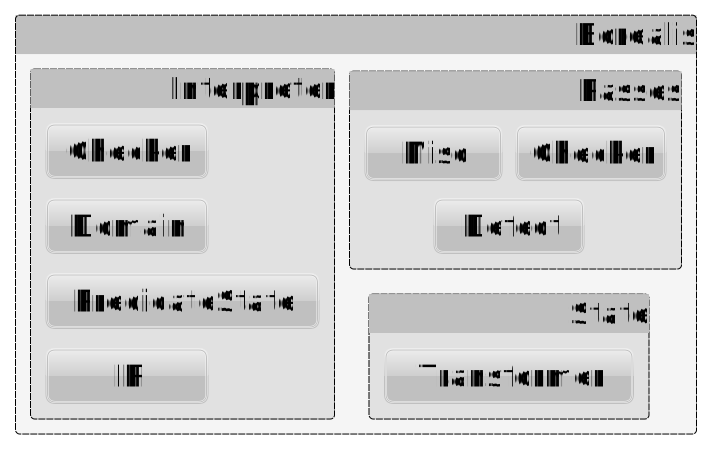
\includegraphics[width=0.8\linewidth]{prototypeArchitecture}}
\caption{Структура разрабатываемого прототипа}
\label{image:prototypeArchitecture}
\end{figure}

Данный модуль основывается на предложенной ранее технологии и содержит реализации
следующих функций: абстрактная интерпретация модуля LLVM, абстрактная 
интерпретация PS, поиск ошибок по результатам интерпретации. Рассмотрим более
подробно все компоненты разрабатываемого модуля.

%%%%%%%%%%%%%%%%%%%%%%%%%%%%%%%%%%%%%%%%%%%%%%%%%%%%%%%%%%%%%%%%%%%%%%%%%%%%%%%
\section{Разработка модуля для системы Borealis}
%%%%%%%%%%%%%%%%%%%%%%%%%%%%%%%%%%%%%%%%%%%%%%%%%%%%%%%%%%%%%%%%%%%%%%%%%%%%%%%
В разработку модуля абстрактной интерпретации для системы Borealis входит 
написание новых классов для анализа кода, а также расширение функциональности 
уже существующих классов. В ходе работы были изменены несколько компонентов 
системы и было реализовано несколько новых компонентов~(см. 
рисунок~\ref{image:prototypeArchitecture}). Компонент \texttt{Interpreter}
содержит реализацию всех классов, связанных с абстрактной интерпретацией:
абстрактных доменов, состояний, интерпретаторов и  т.д. Компонент \texttt{Passes}
содержит проходы LLVM, которые выполняют анализ и модификацию исходного кода.
Компонент \texttt{State} содержит описание и реализацию PS.

%%%%%%%%%%%%%%%%%%%%%%%%%%%%%%%%%%%%%%%%%%%%%%%%%%%%%%%%%%%%%%%%%%%%%%%%%%%%%%%
\subsection{Компонент \texttt{Interpreter}}
%%%%%%%%%%%%%%%%%%%%%%%%%%%%%%%%%%%%%%%%%%%%%%%%%%%%%%%%%%%%%%%%%%%%%%%%%%%%%%%
Компонент \texttt{Interpreter} содержит реализации всех классов, необходимых для
проведения абстрактной интерпретации. В нем содержится два класса: 
\texttt{Interpreter} и \texttt{OneForOneInterpreter}. 

\texttt{Interpreter} --- класс, который выполняет абстрактную интерпретацию 
модуля LLVM~(см. рисунок~\ref{image:irInterpretation}). Он наследуется от класса
\texttt{llvm::InstVisitor}, который реализует шаблон проектирования 
\texttt{Visitor}~\cite{visitor} для инструкций LLVM.

Класс \texttt{OneForOneInterpreter} содержит реализацию метода
\texttt{bool check(PredicateState::Ptr state, PredicateState::Ptr query, const 
DefectInfo\& di)}, который выполняет интерпретацию PS \texttt{state} и 
проверяет, выполняется ли на нем свойство \texttt{query}.

Также, в компоненте \texttt{Interpreter} содержатся следующие пакеты:
\begin{itemize}
\item \texttt{Checker} --- данный пакет содержит реализацию классов, которые 
выполняют поиск ошибок по результатам интерпретации модуля LLVM. Он содержит 
следующие классы:
    \begin{itemize}
    \item \texttt{NullDereferenceChecker} --- класс, для поиска ошибок 
    некорректного разыменовывания указателей~(см. рисунок~\ref{image:ndChecker});
    \item \texttt{OutOfBoundsChecker} --- класс, для поиска ошибок выхода за 
    границы массива~(см. рисунок~\ref{image:oobChecker});
    \item \texttt{OutOfBoundsVisitor} --- вспомогательный класс, который 
    выполняет рекурсивный обход абстрактных доменов для поиска выхода за границы
    массива.
    \end{itemize}
\item \texttt{Domain} --- данный пакет содержит реализации абстрактных доменов для системы типов LLVM~(см. подраздел~\ref{section:domains}). В нем содержатся 
следующие классы:
    \begin{itemize}
    \item \texttt{Domain} --- абстрактный класс абстрактного домена, от которого
    наследуются все абстрактные домены;
    \item \texttt{AggregateDomain} --- реализация агрегатного домена;
    \item \texttt{IntegerIntervalDomain} --- реализация интервального домена для 
    целых чисел;
    \item \texttt{FloatIntervalDomain} --- реализация интервального домена для 
    числе с плавающей точкой;
    \item \texttt{FunctionDomain} --- реализация домена функций;
    \item \texttt{PointerDomain} --- реализация домена указателей;
    \item \texttt{IntervalWidening} --- реализация операторов widening для 
    интервальных доменов;
    \item \texttt{DomainFactory} --- данный класс реализует шаблон 
    проектирования фабрика~\cite{factory} для абстрактных доменов. Также в нем 
    есть методы для разбора константных выражений 
    LLVM~(\texttt{llvm::ConstantExpr}).
    \end{itemize}

    Также в пакете \texttt{Domain} содержатся вспомогательные классы с 
    реализацией решетки целых чисел с фиксированной разрядностью.

\item \texttt{IR} --- в данном пакете содержатся реализации различных 
вспомогательных классов, используемых при интерпретации LLVM IR:
    \begin{itemize}
    \item \texttt{State} --- реализация состояния программы. Для оптимизации 
    использования памяти, было решено хранить в стостоянии программы только
    информацию о локальных переменных. Глобальные переменные было решено
    хранить в единственном экземпляре для всего модуля. Данный класс хранит в 
    себе хэш-таблицу, которая каждой локальной переменной функции ставит в 
    соответствие абстрактный домен, который ее описывает. Так как состояния 
    программы приходится достаточно часто копировать, было решено вместо
    обычной хэш-таблицы использовать в хэш-таблицу, которая копируется только
    при записи~(copy-on-write map);
    \item \texttt{BasicBlock} --- класс-обертка над базовым блоком 
    LLVM~(\texttt{llvm::BasicBlock}), который хранит состояние программы до
    выполнения соответствующего блока и после;
    \item \texttt{Function} --- класс-обертка над функцией 
    LLVM~(\texttt{llvm::Function}), который хранит состояние программы до 
    выполнения функции и после. Также в нем хранится отображение базовых блоков
    LLVM объекты типа \texttt{BasicBlock};
    \item \texttt{Module} --- класс-обертка над модулем программы
    LLVM~(\texttt{llvm::Module}), который хранит информацию о функциях 
    программы;
    \item \texttt{GlobalVariableManager} --- класс, отвечающий за работу с 
    глобальными переменными. Он выполняет топологическую сортировку графа
    глобальных переменных~(глобальные переменные в LLVM могут зависеть друг от
    друга, но при они объявлены в модуле без учета всех зависимостей);
    \item \texttt{ConditionSplitter} --- вспомогательный класс, который 
    выполняет <<разделение>> абстрактных доменов при условных переходах.
    \end{itemize}
\item \texttt{PredicateState}--- в данном пакете содержатся реализации 
различных вспомогательных классов, используемых при интерпретации PS. Он 
содержит в себе два класса:
    \begin{itemize}
    \item \texttt{State} --- состояние программы
    \item \texttt{ConditionSplitter} --- вспомогательный класс, который 
    выполняет <<разделение>> абстрактных доменов при условных переходах в 
    Choice PS.
    \end{itemize}
\end{itemize}